\chapter{Experimentos e resultados}

Neste capítulo serão apresentados os experimentos feitos durante o TCC. Eles tiveram como
finalidade avaliar o uso de métodos e técnica de compressão de modelos, focado em dispositivos
embarcados. Nele serão apresentados os métodos de avaliação do modelo (\autoref{sec_avaliacao_modelo}),

\section{Dispositivo utilizado}\label{sec_dispositivo}
ESP32

\section{Método de avaliação utilizado}\label{sec_avaliacao_modelo}
Para avaliar o modelo, primeiro, as características de cada imagem e sua versão espelhada
(\textit{flip} horizontal) são extraídas pelo modelo. Depois é realizada a verificação da face,
calculando a similaridade de cosseno entre os vetores de características \cite{triplet_distillation_face_recognition}.
% TODO: DETALHAR

\section{Modelo utilizado}\label{sec_modelo_utilizado}
O modelo utilizado foi o mobilefacenet, pois ele mantém uma boa acurácia para detectar as faces enquanto ele necessita
de pouco espaço para ser executado.

---

Neste capítulo serão apresentados testes feitos durante o período inicial do TCC, eles tiveram a finalidade de aplicar técnicas para ter modelos menores.
O objetivo principal é aplicar as técnicas de compressão para criar modelos menores e computacionalmente eficientes.

% Destilação de conhecimento
\section{Destilação de conhecimento (modelo Professor-Aluno)}
Para fazer o experimento com destilação de conhecimento foi utilizada a base STL-10 \cite{stl10}, que possui 500 imagens para
treinamento e 800 para teste, com resolução de $96 \times 96$ e 3 canais de cor (RGB). Como o conjunto de dados
não possui muitas imagens, foi aplicada a técnica de \textit{data augmentation} (aumento de dados) para reduzir o
\textit{overfitting}.

Como já descrito na \autoref{conceitos_destilacao}, o objetivo dessa etapa é utilizar o conhecimento do modelo
Professor (mais robusto e pré-treinado) para treinar o modelo Aluno (mais simples e sem pré-treinamento).
O modelo professor (\autoref{res_professor}) é a ResNet-50  \cite{resnet} e o modelo estudante é gerado pelo
% NOTE: Movo para o texto?
\autoref{res_aluno_1}.
Além disso, o modelo Rafael \cite{rafael} foi adaptado e utilizado (com algumas variações).

% TODO: Continuar correção
Para aumentar a precisão do modelo Aluno com o destilação de conhecimento, foi utilizada a otimização
Bayesiana, para procurar os valores dos hiperparâmetros $\alpha$ e \textit{Temperature}.
% TODO: Revisar
% Talvez mover pro capítulo 02
% Onde $\alpha$ é o peso da \textit{loss function} do modelo estudante e \textit{Temperature} é a relação de
% \textit{logits} da função \textit{softmax}.
Os possíveis valores de $\alpha$ foram 0.1, 0.5, 0.01 e 0.25.
E os possíveis valores de \textit{Temperature} foram 2, 5, 7, 10, 12, 15, 17 e 20.
Os resultados do experimento estão na \autoref{tabela_acuracia_1}.

% TODO: Continuar correção
\begin{center}
\begin{table}[htb]
\centering
\ABNTEXfontereduzida
\caption[Acurácia dos modelos]{Acurácia dos modelos.}
\label{tabela_acuracia_1}
\begin{tabular}{ |c|c|c|c|c| }
	\hline
	\textbf{Modelo} & \textbf{Com destilação de conhecimento?}  & \textbf{Acurácia (validação)}
		   & \textbf{$\alpha$} & \textbf{\textit{Temperature}} \\
	\hline
	% ResNet-50 	& 	Não 	& 	90.65\%	& 	- 	& 	-	 \\
	% Aluno 		& 	Não 	& 	76.80\%	& 	- 	& 	-	 \\
	Rafael-base 	& 	Não 	& 	71.38\%	& 	- 	& 	-	 \\
	Rafael-1 	& 	Não 	& 	67.08\%	& 	- 	& 	-	 \\
	Rafael-2 	& 	Não 	& 	74.57\%	& 	- 	& 	-	 \\
	Rafael-3 	& 	Não 	& 	71.01\%	& 	- 	& 	-	 \\
	% Aluno 		& 	Sim 	& 	83.79\%	& 	0.1 	& 	5	 \\
	Rafael-base 	& 	Sim 	& 	74.21\%	& 	0.1 	& 	10	 \\
	Rafael-1 	& 	Sim 	& 	69.70\%	& 	0.01 	& 	20	 \\
	Rafael-2 	& 	Sim 	& 	79.12\%	& 	0.01 	& 	7	 \\
	Rafael-3 	& 	Sim 	& 	76.55\%	& 	0.01 	& 	5	 \\
	\hline
\end{tabular}
\legend{Fonte: Autor}
\end{table}
\end{center}

A \autoref{tabela_acuracia_1} apresenta a acurácia dos modelos Rafael-Base, Rafael-1, Rafael-2 e Rafael-3 na tarefa de
classificação na base STL-10.
Onde a coluna \textbf{Com destilação de conhecimento?} indica se a técnica de destilação foi aplicada
ou não, e as colunas $\alpha$ e \textit{Temperature} indicam os valores dos hiperparâmetros utilizados.
Percebe-se que, em todos os casos, os modelos que foram treinados utilizando a técnica de destilação de conhecimento alcançaram
uma acurácia maior do que os modelos treinados apenas com os atributos alvo, chegando a um aumento maior que $5\%$ (no modelo
Rafael-3).
Nela, as variações indicam a quantidade de camadas convolucionais adicionadas, Rafael-1
(\autoref{cap_resultados_rafael_1}) indica que foi adicionada uma camada convolucional $9x9$ no modelo, Rafael-2
(\autoref{cap_resultados_rafael_2}) indica que foi adicionada duas camadas $3x3$ convolucionais e Rafael-3
(\autoref{cap_resultados_rafael_3})indica que foi adicionada três camadas $3x3$.

\begin{figure}
	\caption {\label{cap_resultados_rafael_1}Arquitetura do modelo Rafael-1}
	\begin{center}
		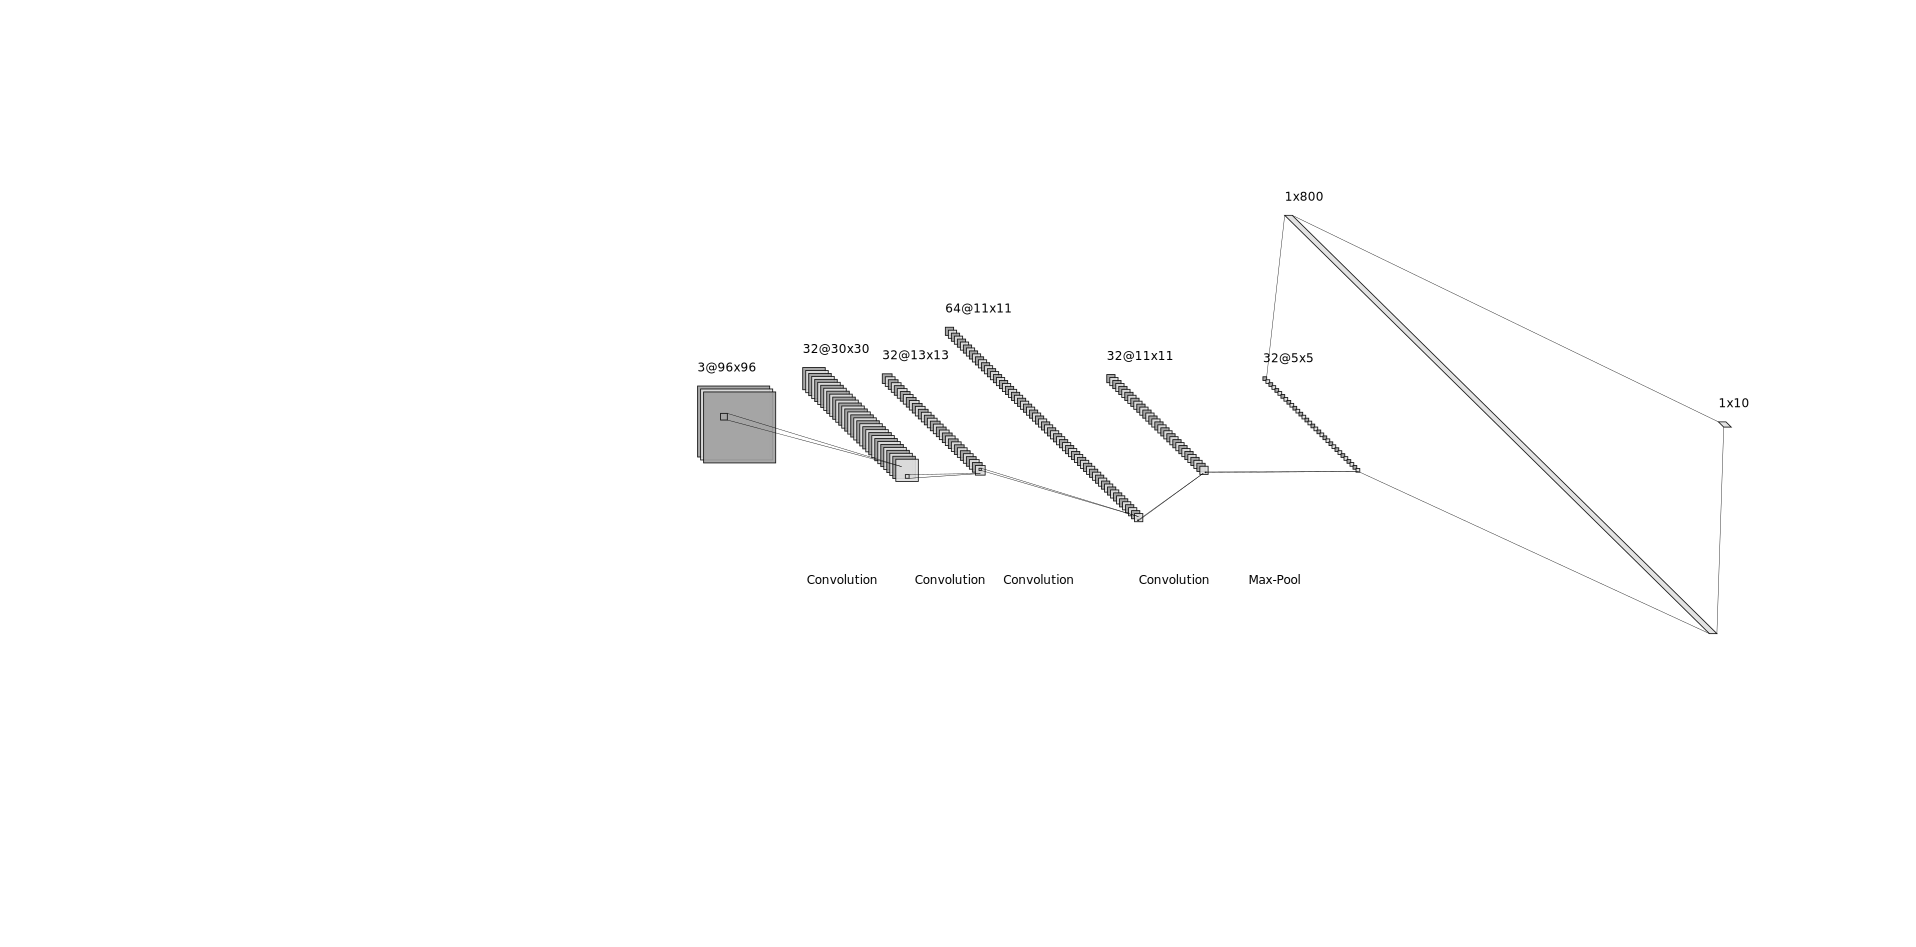
\includegraphics[scale=0.50]{Imagens/arch-rafael-1}
	\end{center}
	\legend {Fonte: Autor}
\end{figure}

\begin{figure}
	\caption {\label{cap_resultados_rafael_2}Arquitetura do modelo Rafael-2}
	\begin{center}
		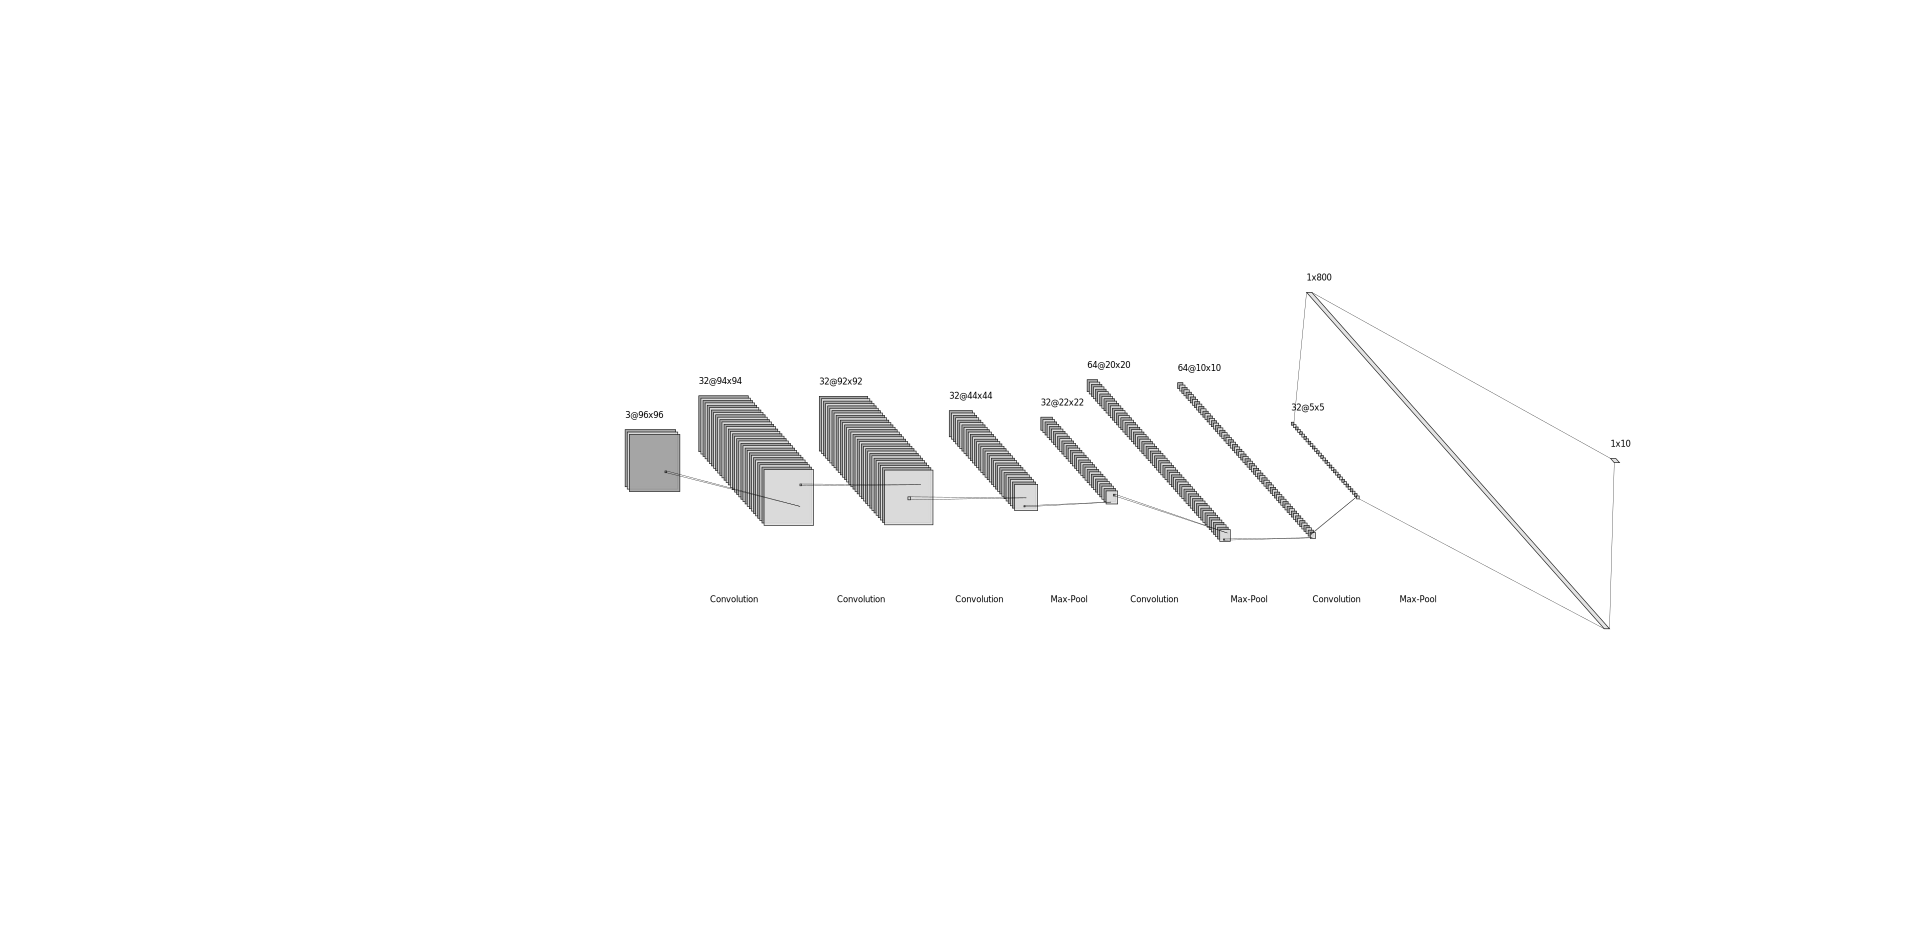
\includegraphics[scale=0.50]{Imagens/arch-rafael-2}
	\end{center}
	\legend {Fonte: Autor}
\end{figure}

\begin{figure}
	\caption {\label{cap_resultados_rafael_3}Arquitetura do modelo Rafael-3}
	\begin{center}
		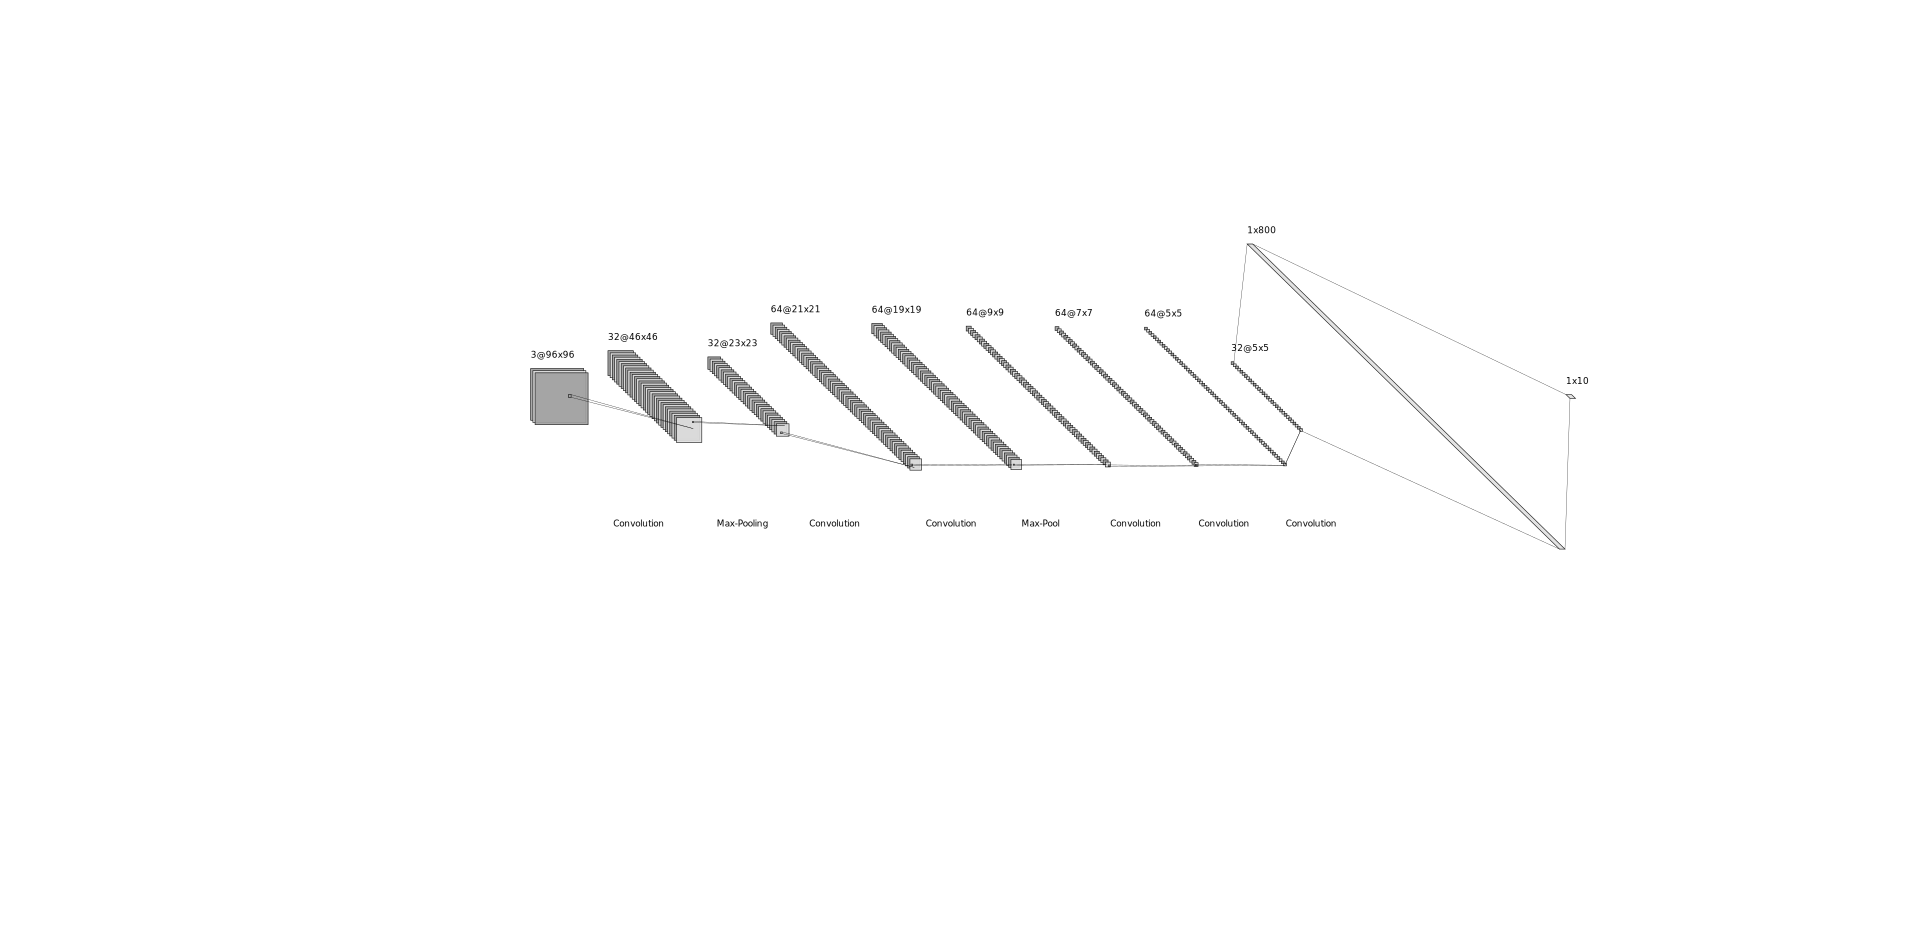
\includegraphics[scale=0.50]{Imagens/arch-rafael-3}
	\end{center}
	\legend {Fonte: Autor}
\end{figure}

\section{\textit{Pruning} e Quantização}

Para esse experimento foi utilizada a base CIFAR-10, pois ela exige menos do modelo, facilitando o treinamento de uma
CNN que performe bem nessa tarefa de classificação, o que permite que o foco da atividade seja mantido.
Essa base possui 10 classes, com  6.000 imagens para cada classe, sendo que essas imagens têm resolução igual a
$32x32$ e possui 3 canais de cores (RGB). Nesse conjunto de dados também foi necessário fazer
\textit{data augmentation} para melhorar a acurácia do modelo final.

O modelo utilizado no experimento foi gerado pelo \autoref{pruning_quantization_model}, inicialmente ele possuía
2.397.226 parâmetros (28 MB). Inicialmente ele foi treinado durante 25 \textit{epochs} (épocas), atingindo
uma acurácia de $90.18\%$ nos dados de treinamento e $85.91\%$ nos dados de validação.
Onde somente os dados de validação serão utilizados para comparar os modelos, pois eles podem sofrer
\textit{overfitting} e ter um alto desempenho nos dados de treinamento e baixo desempenho nos dados de validação.

Depois de treinado, o modelo foi podado utilizando a estratégia de \textit{prune low magnitude}
(podar baixa magnitude), que tem como foco zerar valores abaixo de um certo limiar. Depois de definir os parâmetros da
poda, o modelo foi retreinado por 2 \textit{epochs}, para que o algoritmo de poda consiga identificar as conexões
importantes durante o uso do modelo.
Após o retreinamento, o modelo final teve acurácia de $83.83\%$ nos dados de treinamento e $84.40\%$ nos dados de
validação, consumindo 9.3 MB após remover todos os valores iguais a zero.

Depois de podado, o modelo foi convertido para TensorFlow Lite, consumindo 9.2 MB de armazenamento e ficando com
$84.91\%$ de acurácia. Depois disso, a quantização é aplicada utilizando a API do TensorFlow Lite, deixando o modelo
final com 2.4 MB e $84.36\%$ de acurácia.

\begin{center}
\begin{table}[htb]
\centering
\ABNTEXfontereduzida
\caption[Acurácia e peso dos modelos]{Acurácia e peso dos modelos.}
\label{tabela_acuracia_peso}
\begin{tabular}{ |c|c|c| }
	\hline
	\textbf{Modelo} & \textbf{Acurácia (validação)}  & \textbf{\textit{Memory footprint} (MB)} \\
	\hline
	Modelo base 				 & 	85.91\% 	& 	28	\\
	Modelo base podado 			 & 	84.40\% 	& 	9.3	\\
	Modelo base podado (TFLite) 		 & 	84.91\% 	& 	9.2	\\
	Modelo base podado e quantizado (TFLite) & 	84.36\% 	& 	2.4	\\
	\hline
\end{tabular}
\legend{Fonte: Autor}
\end{table}
\end{center}

A \autoref{tabela_acuracia_peso} mostra a acurácia dos modelos (nos dados de validação) durante as etapas de poda e
quantização, onde a coluna \textbf{\textit{Memory footprint}}  indica o consumo de armazenamento do modelo.
A poda e quantização do modelo base resultou em uma redução de pegada de memória de 28 MB para 2.4 MB, apresentando uma perda
de $1.5\%$ da sua acurácia, tornando o modelo mais eficiente sem a perda de desempenho.
